% FYP M1 report (software track), short form with figures, in the format of the CSE 49x booklet:
% title page per the booklet's example, contents, numbered sections, milestone mapping, "AI Tools Used".
% Build: bash build.sh   (figures are generated from results/published/ by build_figures.py)
\documentclass[11pt,a4paper]{article}
\usepackage[utf8]{inputenc}
\usepackage[T1]{fontenc}
\usepackage{mathpazo}
\usepackage[a4paper,margin=2.5cm]{geometry}
\usepackage{booktabs}
\usepackage{enumitem}
\usepackage{graphicx}
\usepackage{float}
\usepackage{xcolor}
\usepackage{tikz}
\usetikzlibrary{arrows.meta,decorations.pathreplacing}
\usepackage{url}
\urlstyle{tt}
\usepackage{fancyhdr}
\usepackage[hidelinks]{hyperref}
\usepackage[font=small,labelfont=bf]{caption}
\setlist{itemsep=1pt,topsep=3pt}
\pagestyle{fancy}
\fancyhf{}
\fancyhead[L]{\itshape Beyond MCPs: M1 report}
\fancyhead[R]{\thepage}
\renewcommand{\headrulewidth}{0.4pt}
\setlength{\parskip}{3pt}

% colours: IBA maroon and gold, neutral greys; pass/fail tints for the grid
\definecolor{brand}{HTML}{8C2338}
\definecolor{scriptc}{HTML}{A9AEB6}
\definecolor{rulesc}{HTML}{B8862F}
\definecolor{barec}{HTML}{4B5563}
\definecolor{checkc}{HTML}{7A6A8A}
\definecolor{fullc}{HTML}{6B1A2A}
\definecolor{slatec}{HTML}{4A5568}
\definecolor{slatec2}{HTML}{6B6F78}
\definecolor{tintc}{HTML}{F6F1F0}
\definecolor{passc}{HTML}{DDEFE8}
\definecolor{passt}{HTML}{1F5E4F}
\definecolor{failc}{HTML}{F8E3D3}
\definecolor{midc}{HTML}{FBEFD5}
\definecolor{failt}{HTML}{8A3B0B}

% generated by build_figures.py: do not edit
\newcommand{\FigGlance}{\begin{figure}[ht]\centering
\resizebox{\textwidth}{!}{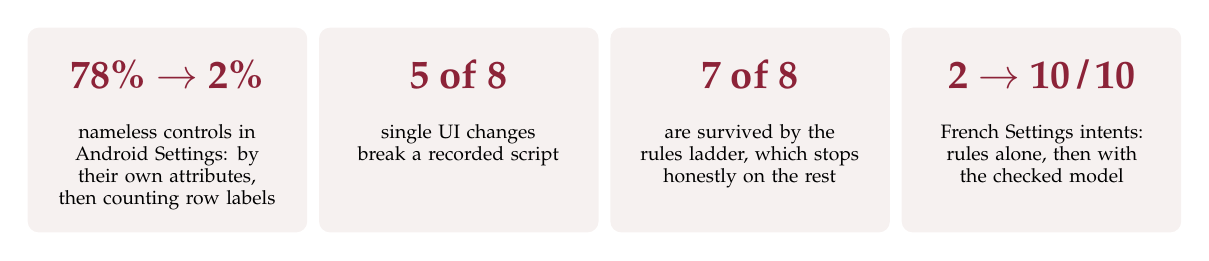
\begin{tikzpicture}[x=1cm,y=1cm,font=\small]
\fill[tintc,rounded corners=4pt] (0.00,0) rectangle (3.55,2.6);
\node[font=\Large\bfseries,text=brand] at (1.77,2.0) {78\% $\rightarrow$ 2\%};
\node[font=\scriptsize,align=center,text width=3.05cm,anchor=north] at (1.77,1.5) {nameless controls in Android Settings: by their own attributes, then counting row labels};
\fill[tintc,rounded corners=4pt] (3.70,0) rectangle (7.25,2.6);
\node[font=\Large\bfseries,text=brand] at (5.47,2.0) {5 of 8};
\node[font=\scriptsize,align=center,text width=3.05cm,anchor=north] at (5.47,1.5) {single UI changes break a recorded script};
\fill[tintc,rounded corners=4pt] (7.40,0) rectangle (10.95,2.6);
\node[font=\Large\bfseries,text=brand] at (9.17,2.0) {7 of 8};
\node[font=\scriptsize,align=center,text width=3.05cm,anchor=north] at (9.17,1.5) {are survived by the rules ladder, which stops honestly on the rest};
\fill[tintc,rounded corners=4pt] (11.10,0) rectangle (14.65,2.6);
\node[font=\Large\bfseries,text=brand] at (12.88,2.0) {2 $\rightarrow$ 10\,/\,10};
\node[font=\scriptsize,align=center,text width=3.05cm,anchor=north] at (12.88,1.5) {French Settings intents: rules alone, then with the checked model};
\end{tikzpicture}}
\caption{At a glance. Every figure is read from the published logs or the coverage measurement.}\label{fig:glance}
\end{figure}
}
\newcommand{\FigRules}{\begin{figure}[ht]\centering
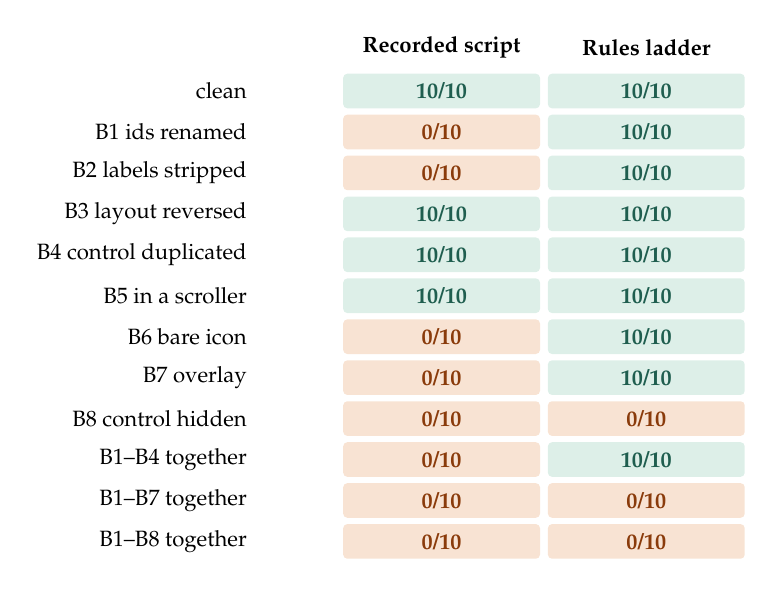
\begin{tikzpicture}[x=1cm,y=1cm,font=\small]
\node[font=\footnotesize\bfseries] at (2.35,0.55) {Recorded script};
\node[font=\footnotesize\bfseries] at (4.95,0.55) {Rules ladder};
\node[anchor=east,font=\footnotesize] at (0.0,0.00) {clean};
\fill[passc,rounded corners=1.5pt] (1.10,-0.22) rectangle (3.60,0.22);
\node[passt,font=\footnotesize\bfseries] at (2.35,0.00) {10/10};
\fill[passc,rounded corners=1.5pt] (3.70,-0.22) rectangle (6.20,0.22);
\node[passt,font=\footnotesize\bfseries] at (4.95,0.00) {10/10};
\node[anchor=east,font=\footnotesize] at (0.0,-0.52) {B1 ids renamed};
\fill[failc,rounded corners=1.5pt] (1.10,-0.74) rectangle (3.60,-0.30);
\node[failt,font=\footnotesize\bfseries] at (2.35,-0.52) {0/10};
\fill[passc,rounded corners=1.5pt] (3.70,-0.74) rectangle (6.20,-0.30);
\node[passt,font=\footnotesize\bfseries] at (4.95,-0.52) {10/10};
\node[anchor=east,font=\footnotesize] at (0.0,-1.04) {B2 labels stripped};
\fill[failc,rounded corners=1.5pt] (1.10,-1.26) rectangle (3.60,-0.82);
\node[failt,font=\footnotesize\bfseries] at (2.35,-1.04) {0/10};
\fill[passc,rounded corners=1.5pt] (3.70,-1.26) rectangle (6.20,-0.82);
\node[passt,font=\footnotesize\bfseries] at (4.95,-1.04) {10/10};
\node[anchor=east,font=\footnotesize] at (0.0,-1.56) {B3 layout reversed};
\fill[passc,rounded corners=1.5pt] (1.10,-1.78) rectangle (3.60,-1.34);
\node[passt,font=\footnotesize\bfseries] at (2.35,-1.56) {10/10};
\fill[passc,rounded corners=1.5pt] (3.70,-1.78) rectangle (6.20,-1.34);
\node[passt,font=\footnotesize\bfseries] at (4.95,-1.56) {10/10};
\node[anchor=east,font=\footnotesize] at (0.0,-2.08) {B4 control duplicated};
\fill[passc,rounded corners=1.5pt] (1.10,-2.30) rectangle (3.60,-1.86);
\node[passt,font=\footnotesize\bfseries] at (2.35,-2.08) {10/10};
\fill[passc,rounded corners=1.5pt] (3.70,-2.30) rectangle (6.20,-1.86);
\node[passt,font=\footnotesize\bfseries] at (4.95,-2.08) {10/10};
\node[anchor=east,font=\footnotesize] at (0.0,-2.60) {B5 in a scroller};
\fill[passc,rounded corners=1.5pt] (1.10,-2.82) rectangle (3.60,-2.38);
\node[passt,font=\footnotesize\bfseries] at (2.35,-2.60) {10/10};
\fill[passc,rounded corners=1.5pt] (3.70,-2.82) rectangle (6.20,-2.38);
\node[passt,font=\footnotesize\bfseries] at (4.95,-2.60) {10/10};
\node[anchor=east,font=\footnotesize] at (0.0,-3.12) {B6 bare icon};
\fill[failc,rounded corners=1.5pt] (1.10,-3.34) rectangle (3.60,-2.90);
\node[failt,font=\footnotesize\bfseries] at (2.35,-3.12) {0/10};
\fill[passc,rounded corners=1.5pt] (3.70,-3.34) rectangle (6.20,-2.90);
\node[passt,font=\footnotesize\bfseries] at (4.95,-3.12) {10/10};
\node[anchor=east,font=\footnotesize] at (0.0,-3.64) {B7 overlay};
\fill[failc,rounded corners=1.5pt] (1.10,-3.86) rectangle (3.60,-3.42);
\node[failt,font=\footnotesize\bfseries] at (2.35,-3.64) {0/10};
\fill[passc,rounded corners=1.5pt] (3.70,-3.86) rectangle (6.20,-3.42);
\node[passt,font=\footnotesize\bfseries] at (4.95,-3.64) {10/10};
\node[anchor=east,font=\footnotesize] at (0.0,-4.16) {B8 control hidden};
\fill[failc,rounded corners=1.5pt] (1.10,-4.38) rectangle (3.60,-3.94);
\node[failt,font=\footnotesize\bfseries] at (2.35,-4.16) {0/10};
\fill[failc,rounded corners=1.5pt] (3.70,-4.38) rectangle (6.20,-3.94);
\node[failt,font=\footnotesize\bfseries] at (4.95,-4.16) {0/10};
\node[anchor=east,font=\footnotesize] at (0.0,-4.68) {B1--B4 together};
\fill[failc,rounded corners=1.5pt] (1.10,-4.90) rectangle (3.60,-4.46);
\node[failt,font=\footnotesize\bfseries] at (2.35,-4.68) {0/10};
\fill[passc,rounded corners=1.5pt] (3.70,-4.90) rectangle (6.20,-4.46);
\node[passt,font=\footnotesize\bfseries] at (4.95,-4.68) {10/10};
\node[anchor=east,font=\footnotesize] at (0.0,-5.20) {B1--B7 together};
\fill[failc,rounded corners=1.5pt] (1.10,-5.42) rectangle (3.60,-4.98);
\node[failt,font=\footnotesize\bfseries] at (2.35,-5.20) {0/10};
\fill[failc,rounded corners=1.5pt] (3.70,-5.42) rectangle (6.20,-4.98);
\node[failt,font=\footnotesize\bfseries] at (4.95,-5.20) {0/10};
\node[anchor=east,font=\footnotesize] at (0.0,-5.72) {B1--B8 together};
\fill[failc,rounded corners=1.5pt] (1.10,-5.94) rectangle (3.60,-5.50);
\node[failt,font=\footnotesize\bfseries] at (2.35,-5.72) {0/10};
\fill[failc,rounded corners=1.5pt] (3.70,-5.94) rectangle (6.20,-5.50);
\node[failt,font=\footnotesize\bfseries] at (4.95,-5.72) {0/10};
\end{tikzpicture}
\caption{Rules only, no model: flows completed out of 10 for the recorded script and the rules ladder under each UI change.}\label{fig:rules}
\end{figure}
}
\newcommand{\FigSemantic}{\begin{figure}[ht]\centering
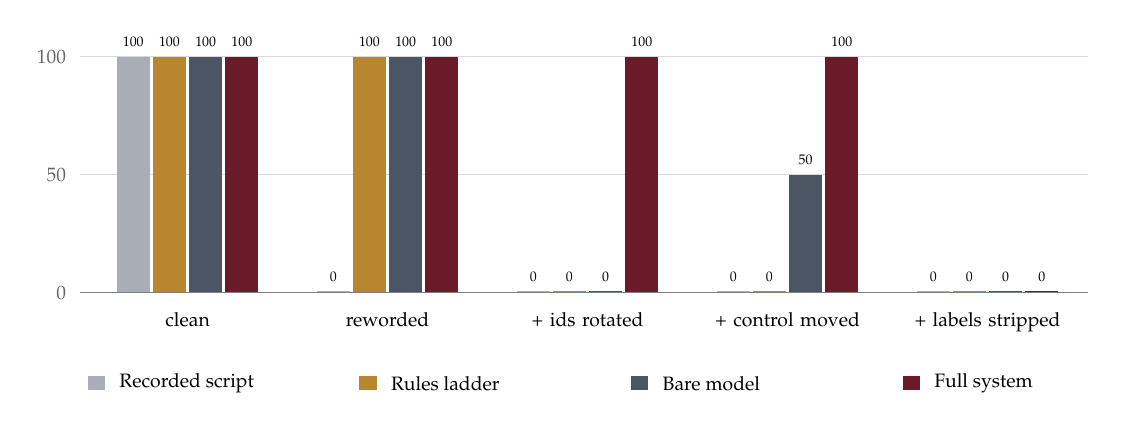
\begin{tikzpicture}[x=1cm,y=1cm,font=\small]
\draw[black!15] (-0.1,0.00) -- (12.70,0.00);
\node[anchor=east,font=\scriptsize,black!60] at (-0.15,0.00) {0};
\draw[black!15] (-0.1,1.50) -- (12.70,1.50);
\node[anchor=east,font=\scriptsize,black!60] at (-0.15,1.50) {50};
\draw[black!15] (-0.1,3.00) -- (12.70,3.00);
\node[anchor=east,font=\scriptsize,black!60] at (-0.15,3.00) {100};
\fill[scriptc] (0.37,0) rectangle (0.79,3.00);
\node[font=\tiny,anchor=south] at (0.58,3.00) {100};
\fill[rulesc] (0.83,0) rectangle (1.25,3.00);
\node[font=\tiny,anchor=south] at (1.04,3.00) {100};
\fill[barec] (1.29,0) rectangle (1.71,3.00);
\node[font=\tiny,anchor=south] at (1.50,3.00) {100};
\fill[fullc] (1.75,0) rectangle (2.17,3.00);
\node[font=\tiny,anchor=south] at (1.96,3.00) {100};
\node[font=\scriptsize,align=center,text width=2.44cm,anchor=north] at (1.27,-0.12) {clean};
\fill[scriptc] (2.91,0) rectangle (3.33,0.02);
\node[font=\tiny,anchor=south] at (3.12,0.02) {0};
\fill[rulesc] (3.37,0) rectangle (3.79,3.00);
\node[font=\tiny,anchor=south] at (3.58,3.00) {100};
\fill[barec] (3.83,0) rectangle (4.25,3.00);
\node[font=\tiny,anchor=south] at (4.04,3.00) {100};
\fill[fullc] (4.29,0) rectangle (4.71,3.00);
\node[font=\tiny,anchor=south] at (4.50,3.00) {100};
\node[font=\scriptsize,align=center,text width=2.44cm,anchor=north] at (3.81,-0.12) {reworded};
\fill[scriptc] (5.45,0) rectangle (5.87,0.02);
\node[font=\tiny,anchor=south] at (5.66,0.02) {0};
\fill[rulesc] (5.91,0) rectangle (6.33,0.02);
\node[font=\tiny,anchor=south] at (6.12,0.02) {0};
\fill[barec] (6.37,0) rectangle (6.79,0.02);
\node[font=\tiny,anchor=south] at (6.58,0.02) {0};
\fill[fullc] (6.83,0) rectangle (7.25,3.00);
\node[font=\tiny,anchor=south] at (7.04,3.00) {100};
\node[font=\scriptsize,align=center,text width=2.44cm,anchor=north] at (6.35,-0.12) {+ ids rotated};
\fill[scriptc] (7.99,0) rectangle (8.41,0.02);
\node[font=\tiny,anchor=south] at (8.20,0.02) {0};
\fill[rulesc] (8.45,0) rectangle (8.87,0.02);
\node[font=\tiny,anchor=south] at (8.66,0.02) {0};
\fill[barec] (8.91,0) rectangle (9.33,1.50);
\node[font=\tiny,anchor=south] at (9.12,1.50) {50};
\fill[fullc] (9.37,0) rectangle (9.79,3.00);
\node[font=\tiny,anchor=south] at (9.58,3.00) {100};
\node[font=\scriptsize,align=center,text width=2.44cm,anchor=north] at (8.89,-0.12) {+ control moved};
\fill[scriptc] (10.53,0) rectangle (10.95,0.02);
\node[font=\tiny,anchor=south] at (10.74,0.02) {0};
\fill[rulesc] (10.99,0) rectangle (11.41,0.02);
\node[font=\tiny,anchor=south] at (11.20,0.02) {0};
\fill[barec] (11.45,0) rectangle (11.87,0.02);
\node[font=\tiny,anchor=south] at (11.66,0.02) {0};
\fill[fullc] (11.91,0) rectangle (12.33,0.02);
\node[font=\tiny,anchor=south] at (12.12,0.02) {0};
\node[font=\scriptsize,align=center,text width=2.44cm,anchor=north] at (11.43,-0.12) {+ labels stripped};
\draw[black!50] (-0.1,0) -- (12.70,0);
\fill[scriptc] (0.00,-1.24) rectangle (0.22,-1.06);
\node[anchor=west,font=\scriptsize] at (0.28,-1.15) {Recorded script};
\fill[rulesc] (3.45,-1.24) rectangle (3.67,-1.06);
\node[anchor=west,font=\scriptsize] at (3.73,-1.15) {Rules ladder};
\fill[barec] (6.90,-1.24) rectangle (7.12,-1.06);
\node[anchor=west,font=\scriptsize] at (7.18,-1.15) {Bare model};
\fill[fullc] (10.35,-1.24) rectangle (10.57,-1.06);
\node[anchor=west,font=\scriptsize] at (10.63,-1.15) {Full system};
\end{tikzpicture}
\caption{Drift the rules cannot read, model qwen3.7-flash: percentage of 10 flows completed. The full system completes until the control is also moved and its label stripped, where no arm completes.}\label{fig:semantic}
\end{figure}
}
\newcommand{\FigInject}{\begin{figure}[ht]\centering
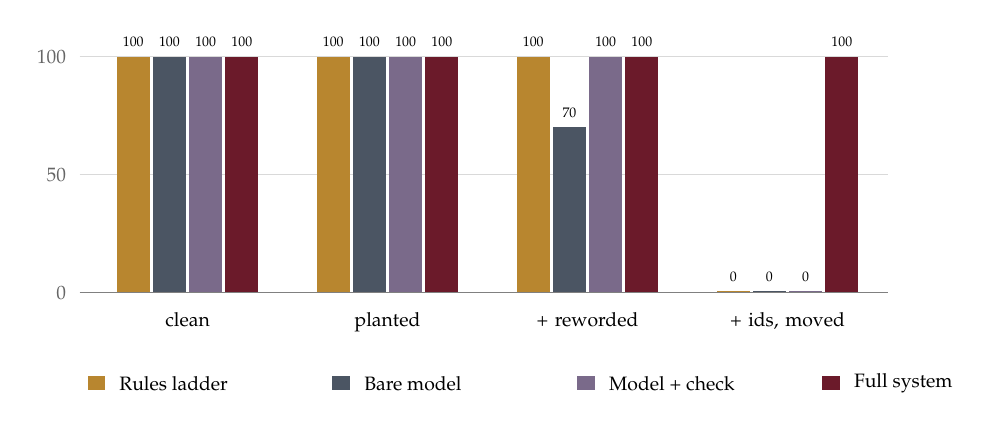
\begin{tikzpicture}[x=1cm,y=1cm,font=\small]
\draw[black!15] (-0.1,0.00) -- (10.16,0.00);
\node[anchor=east,font=\scriptsize,black!60] at (-0.15,0.00) {0};
\draw[black!15] (-0.1,1.50) -- (10.16,1.50);
\node[anchor=east,font=\scriptsize,black!60] at (-0.15,1.50) {50};
\draw[black!15] (-0.1,3.00) -- (10.16,3.00);
\node[anchor=east,font=\scriptsize,black!60] at (-0.15,3.00) {100};
\fill[rulesc] (0.37,0) rectangle (0.79,3.00);
\node[font=\tiny,anchor=south] at (0.58,3.00) {100};
\fill[barec] (0.83,0) rectangle (1.25,3.00);
\node[font=\tiny,anchor=south] at (1.04,3.00) {100};
\fill[checkc] (1.29,0) rectangle (1.71,3.00);
\node[font=\tiny,anchor=south] at (1.50,3.00) {100};
\fill[fullc] (1.75,0) rectangle (2.17,3.00);
\node[font=\tiny,anchor=south] at (1.96,3.00) {100};
\node[font=\scriptsize,align=center,text width=2.44cm,anchor=north] at (1.27,-0.12) {clean};
\fill[rulesc] (2.91,0) rectangle (3.33,3.00);
\node[font=\tiny,anchor=south] at (3.12,3.00) {100};
\fill[barec] (3.37,0) rectangle (3.79,3.00);
\node[font=\tiny,anchor=south] at (3.58,3.00) {100};
\fill[checkc] (3.83,0) rectangle (4.25,3.00);
\node[font=\tiny,anchor=south] at (4.04,3.00) {100};
\fill[fullc] (4.29,0) rectangle (4.71,3.00);
\node[font=\tiny,anchor=south] at (4.50,3.00) {100};
\node[font=\scriptsize,align=center,text width=2.44cm,anchor=north] at (3.81,-0.12) {planted};
\fill[rulesc] (5.45,0) rectangle (5.87,3.00);
\node[font=\tiny,anchor=south] at (5.66,3.00) {100};
\fill[barec] (5.91,0) rectangle (6.33,2.10);
\node[font=\tiny,anchor=south] at (6.12,2.10) {70};
\fill[checkc] (6.37,0) rectangle (6.79,3.00);
\node[font=\tiny,anchor=south] at (6.58,3.00) {100};
\fill[fullc] (6.83,0) rectangle (7.25,3.00);
\node[font=\tiny,anchor=south] at (7.04,3.00) {100};
\node[font=\scriptsize,align=center,text width=2.44cm,anchor=north] at (6.35,-0.12) {+ reworded};
\fill[rulesc] (7.99,0) rectangle (8.41,0.02);
\node[font=\tiny,anchor=south] at (8.20,0.02) {0};
\fill[barec] (8.45,0) rectangle (8.87,0.02);
\node[font=\tiny,anchor=south] at (8.66,0.02) {0};
\fill[checkc] (8.91,0) rectangle (9.33,0.02);
\node[font=\tiny,anchor=south] at (9.12,0.02) {0};
\fill[fullc] (9.37,0) rectangle (9.79,3.00);
\node[font=\tiny,anchor=south] at (9.58,3.00) {100};
\node[font=\scriptsize,align=center,text width=2.44cm,anchor=north] at (8.89,-0.12) {+ ids, moved};
\draw[black!50] (-0.1,0) -- (10.16,0);
\fill[rulesc] (0.00,-1.24) rectangle (0.22,-1.06);
\node[anchor=west,font=\scriptsize] at (0.28,-1.15) {Rules ladder};
\fill[barec] (3.11,-1.24) rectangle (3.33,-1.06);
\node[anchor=west,font=\scriptsize] at (3.39,-1.15) {Bare model};
\fill[checkc] (6.22,-1.24) rectangle (6.44,-1.06);
\node[anchor=west,font=\scriptsize] at (6.50,-1.15) {Model + check};
\fill[fullc] (9.33,-1.24) rectangle (9.55,-1.06);
\node[anchor=west,font=\scriptsize] at (9.61,-1.15) {Full system};
\end{tikzpicture}
\caption{Instructions planted in control labels (B11), model qwen3.7-flash: percentage of 10 flows completed. The bare model fails three of ten when the labels are also reworded; the full system completes the hardest case, tapping a planted label twice per run on the way and recovering through the step check.}\label{fig:inject}
\end{figure}
}
\newcommand{\FigVision}{\begin{figure}[ht]\centering
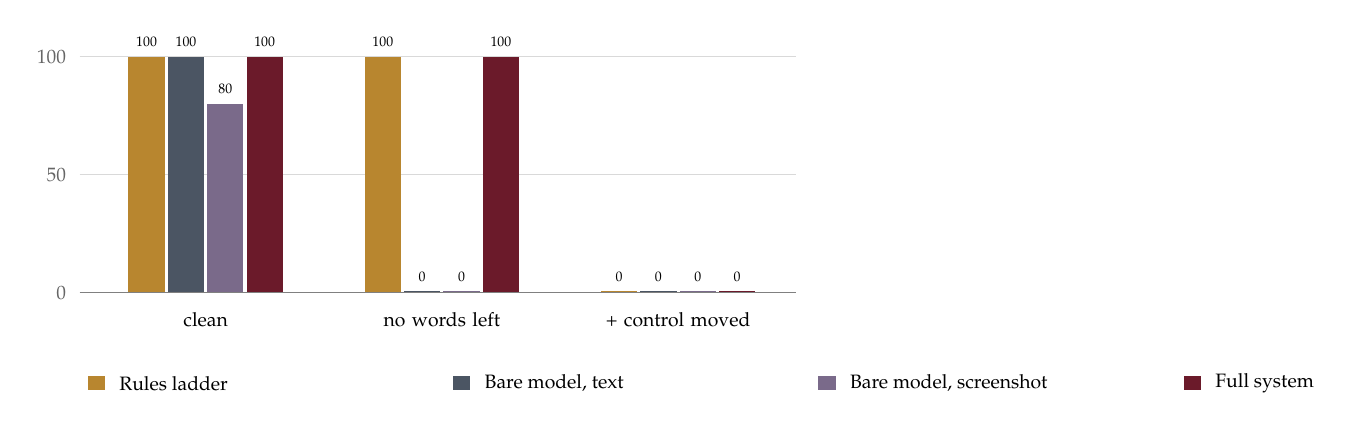
\begin{tikzpicture}[x=1cm,y=1cm,font=\small]
\draw[black!15] (-0.1,0.00) -- (9.00,0.00);
\node[anchor=east,font=\scriptsize,black!60] at (-0.15,0.00) {0};
\draw[black!15] (-0.1,1.50) -- (9.00,1.50);
\node[anchor=east,font=\scriptsize,black!60] at (-0.15,1.50) {50};
\draw[black!15] (-0.1,3.00) -- (9.00,3.00);
\node[anchor=east,font=\scriptsize,black!60] at (-0.15,3.00) {100};
\fill[rulesc] (0.52,0) rectangle (0.98,3.00);
\node[font=\tiny,anchor=south] at (0.75,3.00) {100};
\fill[barec] (1.02,0) rectangle (1.48,3.00);
\node[font=\tiny,anchor=south] at (1.25,3.00) {100};
\fill[checkc] (1.52,0) rectangle (1.98,2.40);
\node[font=\tiny,anchor=south] at (1.75,2.40) {80};
\fill[fullc] (2.02,0) rectangle (2.48,3.00);
\node[font=\tiny,anchor=south] at (2.25,3.00) {100};
\node[font=\scriptsize,align=center,text width=2.90cm,anchor=north] at (1.50,-0.12) {clean};
\fill[rulesc] (3.52,0) rectangle (3.98,3.00);
\node[font=\tiny,anchor=south] at (3.75,3.00) {100};
\fill[barec] (4.02,0) rectangle (4.48,0.02);
\node[font=\tiny,anchor=south] at (4.25,0.02) {0};
\fill[checkc] (4.52,0) rectangle (4.98,0.02);
\node[font=\tiny,anchor=south] at (4.75,0.02) {0};
\fill[fullc] (5.02,0) rectangle (5.48,3.00);
\node[font=\tiny,anchor=south] at (5.25,3.00) {100};
\node[font=\scriptsize,align=center,text width=2.90cm,anchor=north] at (4.50,-0.12) {no words left};
\fill[rulesc] (6.52,0) rectangle (6.98,0.02);
\node[font=\tiny,anchor=south] at (6.75,0.02) {0};
\fill[barec] (7.02,0) rectangle (7.48,0.02);
\node[font=\tiny,anchor=south] at (7.25,0.02) {0};
\fill[checkc] (7.52,0) rectangle (7.98,0.02);
\node[font=\tiny,anchor=south] at (7.75,0.02) {0};
\fill[fullc] (8.02,0) rectangle (8.48,0.02);
\node[font=\tiny,anchor=south] at (8.25,0.02) {0};
\node[font=\scriptsize,align=center,text width=2.90cm,anchor=north] at (7.50,-0.12) {+ control moved};
\draw[black!50] (-0.1,0) -- (9.00,0);
\fill[rulesc] (0.00,-1.24) rectangle (0.22,-1.06);
\node[anchor=west,font=\scriptsize] at (0.28,-1.15) {Rules ladder};
\fill[barec] (4.64,-1.24) rectangle (4.86,-1.06);
\node[anchor=west,font=\scriptsize] at (4.92,-1.15) {Bare model, text};
\fill[checkc] (9.28,-1.24) rectangle (9.50,-1.06);
\node[anchor=west,font=\scriptsize] at (9.56,-1.15) {Bare model, screenshot};
\fill[fullc] (13.92,-1.24) rectangle (14.14,-1.06);
\node[anchor=west,font=\scriptsize] at (14.20,-1.15) {Full system};
\end{tikzpicture}
\caption{No words left on the target (B1, B2, B6), five flows per cell, model qwen3.7-flash: percentage completed. Showing the model a screenshot with numbered badges did not change the outcome in this run.}\label{fig:vision}
\end{figure}
}
\newcommand{\FigAndroid}{\begin{figure}[ht]\centering
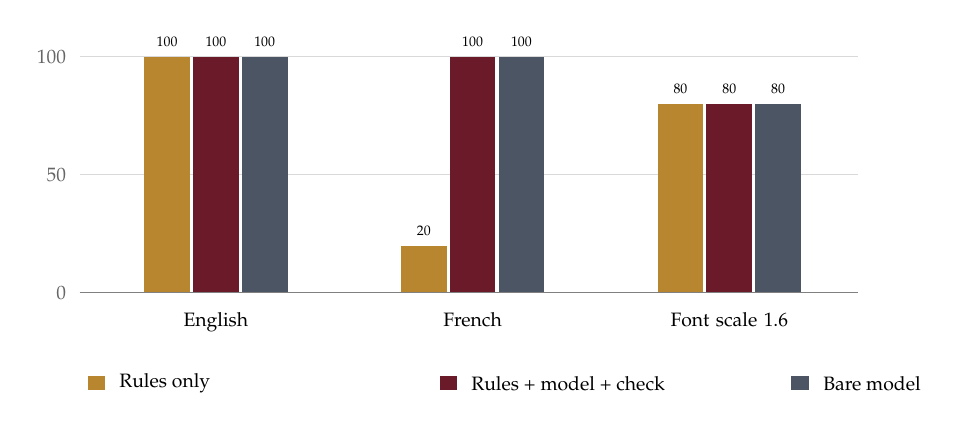
\begin{tikzpicture}[x=1cm,y=1cm,font=\small]
\draw[black!15] (-0.1,0.00) -- (9.78,0.00);
\node[anchor=east,font=\scriptsize,black!60] at (-0.15,0.00) {0};
\draw[black!15] (-0.1,1.50) -- (9.78,1.50);
\node[anchor=east,font=\scriptsize,black!60] at (-0.15,1.50) {50};
\draw[black!15] (-0.1,3.00) -- (9.78,3.00);
\node[anchor=east,font=\scriptsize,black!60] at (-0.15,3.00) {100};
\fill[rulesc] (0.72,0) rectangle (1.30,3.00);
\node[font=\tiny,anchor=south] at (1.01,3.00) {100};
\fill[fullc] (1.34,0) rectangle (1.92,3.00);
\node[font=\tiny,anchor=south] at (1.63,3.00) {100};
\fill[barec] (1.96,0) rectangle (2.54,3.00);
\node[font=\tiny,anchor=south] at (2.25,3.00) {100};
\node[font=\scriptsize,align=center,text width=3.16cm,anchor=north] at (1.63,-0.12) {English};
\fill[rulesc] (3.98,0) rectangle (4.56,0.60);
\node[font=\tiny,anchor=south] at (4.27,0.60) {20};
\fill[fullc] (4.60,0) rectangle (5.18,3.00);
\node[font=\tiny,anchor=south] at (4.89,3.00) {100};
\fill[barec] (5.22,0) rectangle (5.80,3.00);
\node[font=\tiny,anchor=south] at (5.51,3.00) {100};
\node[font=\scriptsize,align=center,text width=3.16cm,anchor=north] at (4.89,-0.12) {French};
\fill[rulesc] (7.24,0) rectangle (7.82,2.40);
\node[font=\tiny,anchor=south] at (7.53,2.40) {80};
\fill[fullc] (7.86,0) rectangle (8.44,2.40);
\node[font=\tiny,anchor=south] at (8.15,2.40) {80};
\fill[barec] (8.48,0) rectangle (9.06,2.40);
\node[font=\tiny,anchor=south] at (8.77,2.40) {80};
\node[font=\scriptsize,align=center,text width=3.16cm,anchor=north] at (8.15,-0.12) {Font scale 1.6};
\draw[black!50] (-0.1,0) -- (9.78,0);
\fill[rulesc] (0.00,-1.24) rectangle (0.22,-1.06);
\node[anchor=west,font=\scriptsize] at (0.28,-1.15) {Rules only};
\fill[fullc] (4.47,-1.24) rectangle (4.69,-1.06);
\node[anchor=west,font=\scriptsize] at (4.75,-1.15) {Rules + model + check};
\fill[barec] (8.94,-1.24) rectangle (9.16,-1.06);
\node[anchor=west,font=\scriptsize] at (9.22,-1.15) {Bare model};
\end{tikzpicture}
\caption{Android Settings, real drift (system language and font scale): percentage of intents completed on the \texttt{kenna} emulator, model qwen3.7-flash. At the large font two rows fall below the fold, which no arm scrolled to.}\label{fig:android}
\end{figure}
}
\newcommand{\FigLearn}{\begin{figure}[ht]\centering
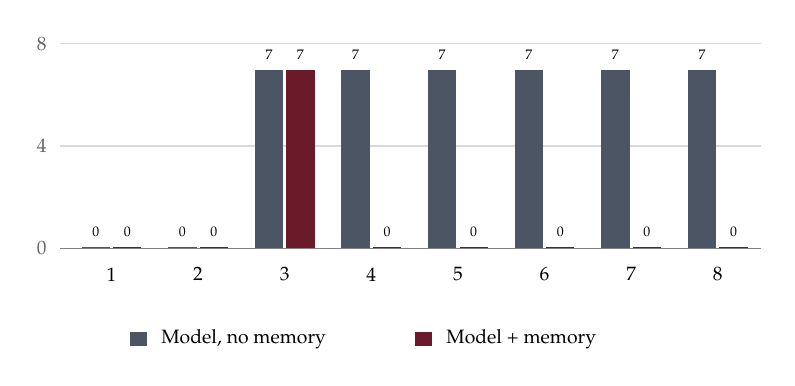
\begin{tikzpicture}[x=1cm,y=1cm,font=\small]
\draw[black!15] (-0.1,0.00) -- (8.80,0.00);
\node[anchor=east,font=\scriptsize,black!60] at (-0.15,0.00) {0};
\draw[black!15] (-0.1,1.30) -- (8.80,1.30);
\node[anchor=east,font=\scriptsize,black!60] at (-0.15,1.30) {4};
\draw[black!15] (-0.1,2.60) -- (8.80,2.60);
\node[anchor=east,font=\scriptsize,black!60] at (-0.15,2.60) {8};
\fill[barec] (0.17,0) rectangle (0.53,0.02);
\node[font=\tiny,anchor=south] at (0.35,0.02) {0};
\fill[fullc] (0.57,0) rectangle (0.93,0.02);
\node[font=\tiny,anchor=south] at (0.75,0.02) {0};
\node[font=\scriptsize,align=center,text width=1.00cm,anchor=north] at (0.55,-0.12) {1};
\fill[barec] (1.27,0) rectangle (1.63,0.02);
\node[font=\tiny,anchor=south] at (1.45,0.02) {0};
\fill[fullc] (1.67,0) rectangle (2.03,0.02);
\node[font=\tiny,anchor=south] at (1.85,0.02) {0};
\node[font=\scriptsize,align=center,text width=1.00cm,anchor=north] at (1.65,-0.12) {2};
\fill[barec] (2.37,0) rectangle (2.73,2.27);
\node[font=\tiny,anchor=south] at (2.55,2.27) {7};
\fill[fullc] (2.77,0) rectangle (3.13,2.27);
\node[font=\tiny,anchor=south] at (2.95,2.27) {7};
\node[font=\scriptsize,align=center,text width=1.00cm,anchor=north] at (2.75,-0.12) {3};
\fill[barec] (3.47,0) rectangle (3.83,2.27);
\node[font=\tiny,anchor=south] at (3.65,2.27) {7};
\fill[fullc] (3.87,0) rectangle (4.23,0.02);
\node[font=\tiny,anchor=south] at (4.05,0.02) {0};
\node[font=\scriptsize,align=center,text width=1.00cm,anchor=north] at (3.85,-0.12) {4};
\fill[barec] (4.57,0) rectangle (4.93,2.27);
\node[font=\tiny,anchor=south] at (4.75,2.27) {7};
\fill[fullc] (4.97,0) rectangle (5.33,0.02);
\node[font=\tiny,anchor=south] at (5.15,0.02) {0};
\node[font=\scriptsize,align=center,text width=1.00cm,anchor=north] at (4.95,-0.12) {5};
\fill[barec] (5.67,0) rectangle (6.03,2.27);
\node[font=\tiny,anchor=south] at (5.85,2.27) {7};
\fill[fullc] (6.07,0) rectangle (6.43,0.02);
\node[font=\tiny,anchor=south] at (6.25,0.02) {0};
\node[font=\scriptsize,align=center,text width=1.00cm,anchor=north] at (6.05,-0.12) {6};
\fill[barec] (6.77,0) rectangle (7.13,2.27);
\node[font=\tiny,anchor=south] at (6.95,2.27) {7};
\fill[fullc] (7.17,0) rectangle (7.53,0.02);
\node[font=\tiny,anchor=south] at (7.35,0.02) {0};
\node[font=\scriptsize,align=center,text width=1.00cm,anchor=north] at (7.15,-0.12) {7};
\fill[barec] (7.87,0) rectangle (8.23,2.27);
\node[font=\tiny,anchor=south] at (8.05,2.27) {7};
\fill[fullc] (8.27,0) rectangle (8.63,0.02);
\node[font=\tiny,anchor=south] at (8.45,0.02) {0};
\node[font=\scriptsize,align=center,text width=1.00cm,anchor=north] at (8.25,-0.12) {8};
\draw[black!50] (-0.1,0) -- (8.80,0);
\fill[barec] (0.78,-1.24) rectangle (1.00,-1.06);
\node[anchor=west,font=\scriptsize] at (1.06,-1.15) {Model, no memory};
\fill[fullc] (4.40,-1.24) rectangle (4.62,-1.06);
\node[anchor=west,font=\scriptsize] at (4.68,-1.15) {Model + memory};
\end{tikzpicture}
\caption{Route memory: model calls per run over 8 runs; the UI changes at run 3. With memory the first run after the change asks the model and later runs do not.}\label{fig:learn}
\end{figure}
}
\newcommand{\FigFlow}{\begin{figure}[ht]\centering
\resizebox{\textwidth}{!}{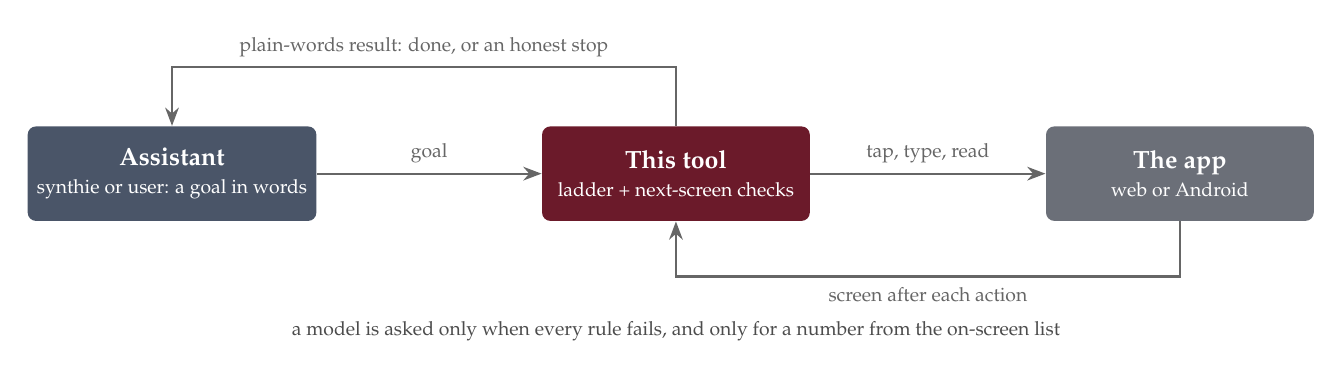
\begin{tikzpicture}[x=1cm,y=1cm,font=\small]

\tikzset{blk/.style={rounded corners=3pt,minimum height=1.2cm,minimum width=3.4cm,text=white,align=center,font=\small}}
\node[blk,fill=slatec] (a) at (0,0) {\textbf{Assistant}\\[-1pt]{\scriptsize synthie or user: a goal in words}};
\node[blk,fill=fullc] (b) at (6.4,0) {\textbf{This tool}\\[-1pt]{\scriptsize ladder + next-screen checks}};
\node[blk,fill=slatec2] (c) at (12.8,0) {\textbf{The app}\\[-1pt]{\scriptsize web or Android}};
\draw[-{Stealth},thick,black!60] (a) -- node[above,font=\scriptsize]{goal} (b);
\draw[-{Stealth},thick,black!60] (b) -- node[above,font=\scriptsize]{tap, type, read} (c);
\draw[-{Stealth},thick,black!60] (c.south) -- ++(0,-0.7) -| node[pos=0.25,below,font=\scriptsize]{screen after each action} (b.south);
\draw[-{Stealth},thick,black!60] (b.north) -- ++(0,0.75) -| node[pos=0.25,above,font=\scriptsize]{plain-words result: done, or an honest stop} (a.north);
\node[font=\scriptsize,align=center,text=black!70] at (6.4,-2.0) {a model is asked only when every rule fails, and only for a number from the on-screen list};
\end{tikzpicture}}
\caption{How the tool sits between an assistant and an app.}\label{fig:flow}
\end{figure}
}
\newcommand{\FigLadder}{\begin{figure}[ht]\centering
\resizebox{\textwidth}{!}{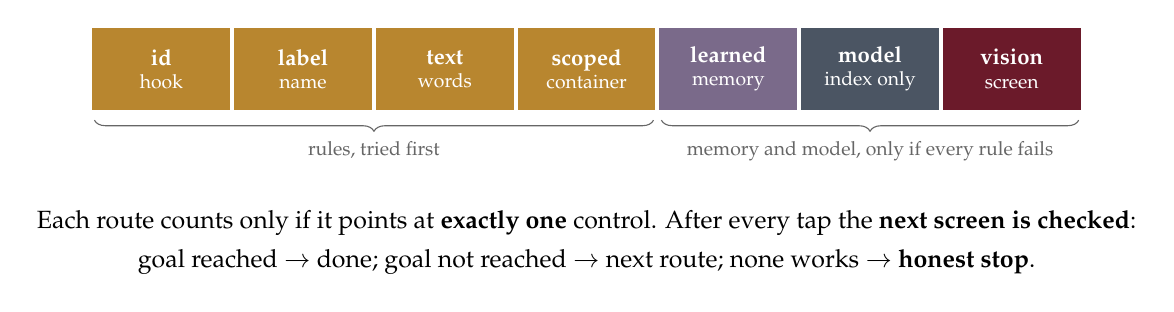
\begin{tikzpicture}[x=1cm,y=1cm,font=\small]

\tikzset{rung/.style={minimum width=1.75cm,minimum height=1.05cm,text=white,align=center,font=\footnotesize}}
\foreach \x/\t/\s/\c in {0/id/hook/rulesc,1.8/label/name/rulesc,3.6/text/words/rulesc,5.4/scoped/container/rulesc,7.2/learned/memory/checkc,9.0/model/index only/barec,10.8/vision/screen/fullc}
  \node[rung,fill=\c] at (\x,0) {\textbf{\t}\\[-1pt]{\scriptsize \s}};
\draw[decorate,decoration={brace,amplitude=4pt,mirror},black!60] (-0.85,-0.65) -- (6.25,-0.65) node[midway,below=4pt,font=\scriptsize]{rules, tried first};
\draw[decorate,decoration={brace,amplitude=4pt,mirror},black!60] (6.35,-0.65) -- (11.65,-0.65) node[midway,below=4pt,font=\scriptsize]{memory and model, only if every rule fails};
\node[font=\small,align=left] at (5.4,-1.95) {Each route counts only if it points at \textbf{exactly one} control.  After every tap the \textbf{next screen is checked}:};
\node[font=\small,align=left] at (5.4,-2.45) {goal reached $\rightarrow$ done; goal not reached $\rightarrow$ next route; none works $\rightarrow$ \textbf{honest stop}.};
\end{tikzpicture}}
\caption{The ladder of ways to find a control, tried left to right.}\label{fig:ladder}
\end{figure}
}


\begin{document}

% ---------------------------------------------------------------- title page (booklet, section 0.5.2)
\begin{titlepage}
\centering
\vspace*{0.8cm}

\includegraphics[height=2.6cm]{../assets/logo-iba.jpg}\par
\vspace{1.6cm}
{\LARGE\bfseries Beyond MCPs\par}
\vspace{4pt}
{\large Self-healing, verified GUI automation for accessible AI assistants\par}
\vspace{1.2cm}
{\Large\scshape M1 report: MVP and proposal\par}
\vspace{4pt}
{\normalsize CSE 493 -- Final Year Project, Term 1 \quad Software track\par}
\vspace{1.4cm}
\begin{tabular}{@{}p{6.2cm}p{6.2cm}@{}}
\textbf{Authors:} & \textbf{Advisors:}\\[4pt]
Sharique Baig (28369) & Dr.\ Faisal Iradat\\
Maira Aijaz (28552) & Pete Herzog (ISECOM)\\
Barkhi Khan (29261) & \\
\end{tabular}
\vfill
October 29, 2026\par
\vspace{6pt}
Department of Computer Science,\\
School of Mathematics and Computer Science,\\
Institute of Business Administration, Karachi
\vspace{1.2cm}
\end{titlepage}

\tableofcontents
\newpage

\section{Context}
Assistants are increasingly asked to operate software through its screen, because many everyday apps expose no API. Where an API or an MCP server exists it should be used; this project is about the apps that offer nothing else. Recorded scripts are the usual tool, and they fail in two ways: one renamed id sends a click nowhere, and a script that never checks the next screen cannot tell that the goal was not reached. For a blind or motor-impaired user, being told ``please do this step yourself'' is not a fallback, so the assistant must be right or say clearly that it is not.

The information a screen reader uses is usually present. On stock Android Settings, 78\% of controls look nameless by their own attributes, but only 2\% are nameless once the labels inside a clickable row are counted (measured with \path{path-b/hierdump.py}).

\FigGlance

\paragraph{Platforms.} Figure~\ref{fig:poster} is the project poster. It sorts platforms into agent-native (APIs and MCP: out of scope), legacy local apps without an API (our target class) and agent-hostile platforms. We evaluated a mock Instagram-style web app and stock Android Settings; Daraz, OLX and Instagram were \emph{not} tested.

\begin{figure}[ht]
\centering
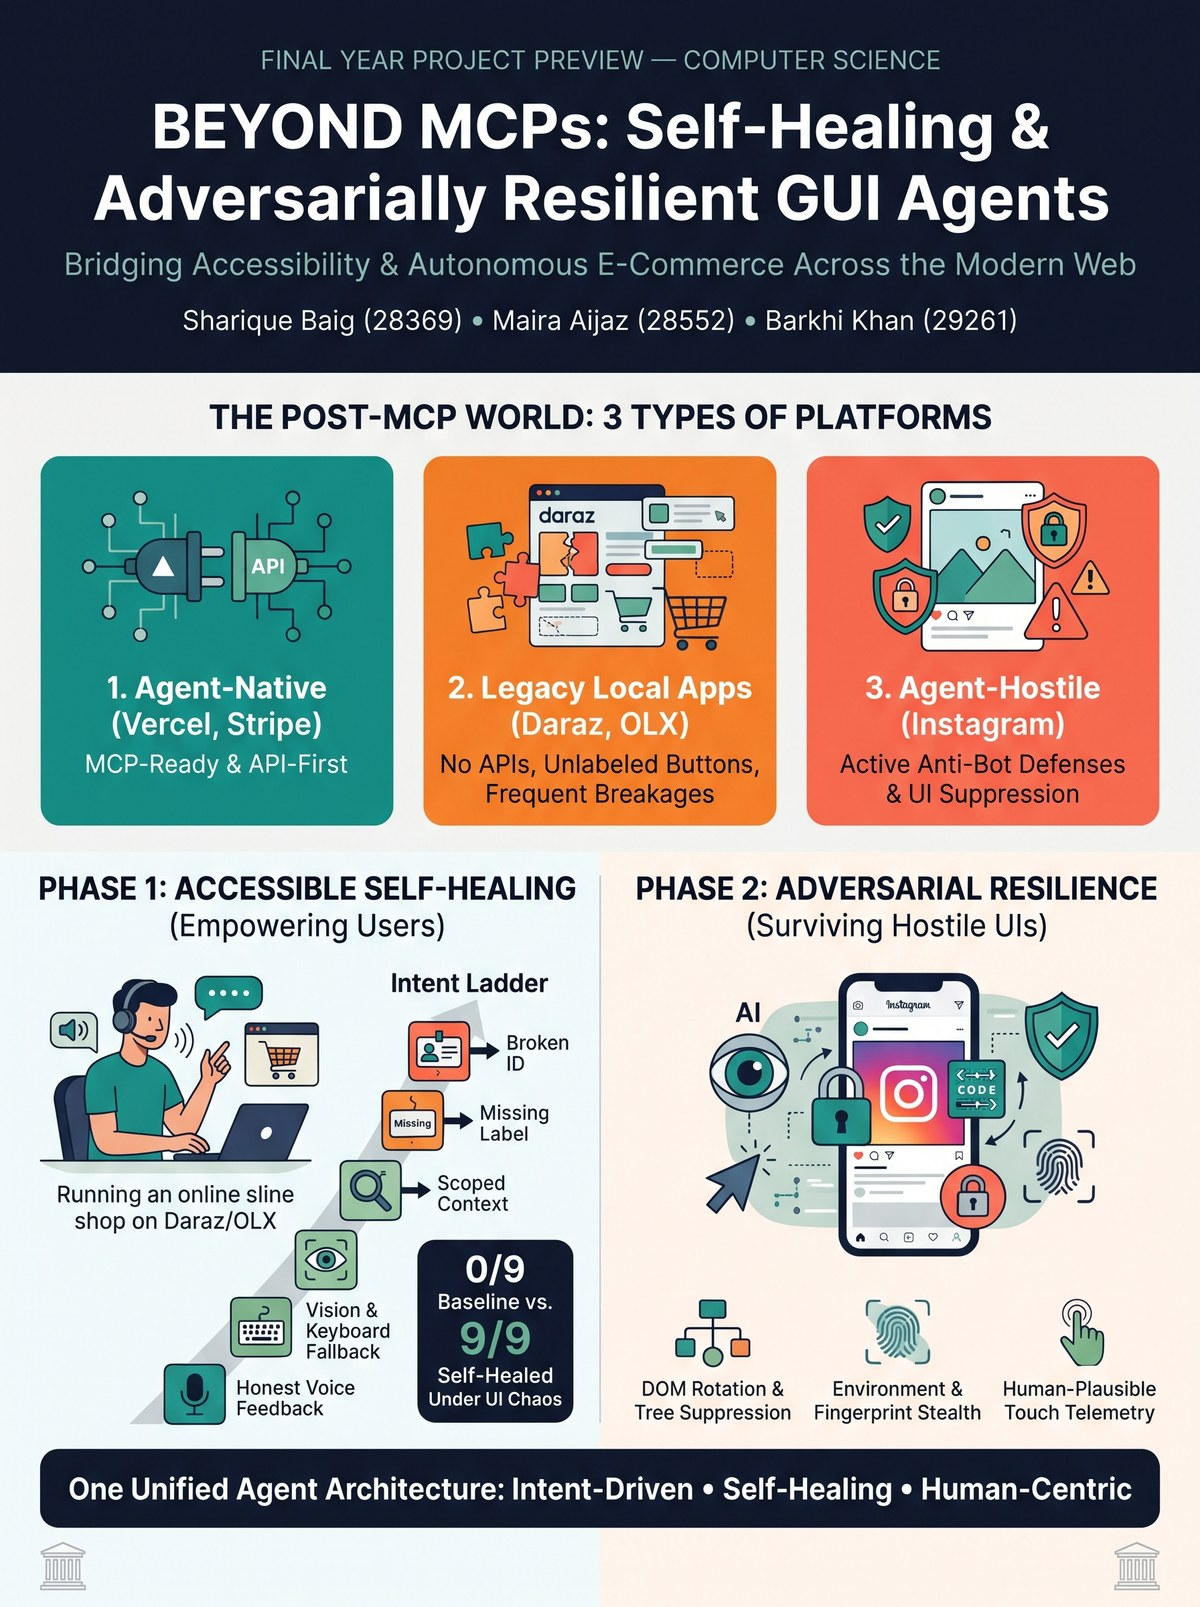
\includegraphics[height=8.2cm]{../presentation/assets/poster.jpg}
\caption{The project poster (earlier wording). Its Phase~2 claims are narrowed by the scope below.}
\label{fig:poster}
\end{figure}

\paragraph{Collaboration.} The advisor is Dr.\ Faisal Iradat. The work started from a scoping brief written by a \emph{synthie} (a long-running agent with its own host, identity and owner) about the failures of its own Android automation, and is carried out with Pete Herzog of the Institute for Security and Open Methodologies (ISECOM), an open security research community that published the OSSTMM in 2001.

\paragraph{Scope.} Surviving anti-bot detection is out of scope: we measure how a protection layer treats an agent and fail honestly, but build no evasion. A model is never trusted with an action (Section~\ref{sec:approach}).

\section{Track and milestone}
The project is on the software track. This report is the M1 checkpoint: a working demonstrator of the core idea and a written proposal.

\begin{table}[H]\centering\small
\begin{tabular}{p{5.2cm}p{8.6cm}}\toprule
M1 requirement & Evidence \\ \midrule
Working demonstrator of the core part & A nine-step flow runs end to end with next-screen checks; an Android layer runs on an emulator. \\
External integration works & Playwright drives a browser; \texttt{adb} drives an emulator; a language model is called through OpenRouter. \\
Written proposal & This report, including the plan in Section~\ref{sec:plan}. \\
AI-tool disclosure & Section~\ref{sec:ai}. \\ \bottomrule
\end{tabular}
\end{table}

\section{Approach}\label{sec:approach}
The tool follows three rules. \textbf{Intent, not locator:} the assistant states a goal such as ``open the create-post flow'', never a button. \textbf{Verify on the next screen:} a step counts only if a predicate on the next screen shows the goal was reached. \textbf{Stop honestly:} if nothing works, the tool says which step failed and why, ending ``You may need to do this step yourself.''

\FigFlow

For each step it tries a ladder of ways to find the control (Figure~\ref{fig:ladder}). The model is asked only when every rule route fails; it may answer only with indices into the on-screen control list, its answer is a candidate judged by the same next-screen check, and an irreversible step (publishing) needs confidence of at least 0.8 and only the first choice. A model answer that passed its check is remembered so the model need not be asked again. The Android layer applies the same ladder to UiAutomator trees and pages a scrollable list when nothing has been tapped and a control may be below the fold. The tool can also say its result aloud, reporting success only when every check passed.

\FigLadder

\section{The demonstrator}
\begin{itemize}
\item \texttt{node agent/fyp.mjs run} performs the nine-step create-post flow on the mock app, verified in the feed; flags select UI changes, the recorded-script arm, the model rung and voice.
\item \texttt{node agent/fyp.mjs experiment} runs arms against UI changes and writes raw logs; reports and figures are built from those logs.
\item \texttt{python path-b/dashboard.py} is a live Android view.
\end{itemize}
A regression set (unit suites, Android self-tests and three end-to-end runs) is run after every change to the harness. It needs only Node~18; there is no GPU requirement.

\section{Evaluation}
\paragraph{Method.} One nine-step flow on the mock app; a flow \emph{completes} only if every step passes its next-screen check. Eleven controlled UI changes (B1--B11: ids renamed, labels stripped, layout reversed, control duplicated, nested in a scroller, bare icon, overlay, hidden, reworded, relocated, planted instructions) are applied alone and together. Arms: a recorded script, the rules ladder, a bare model acting on its first pick, a model with a check but no rules, and the full system. Each cell is 10 runs with 95\% Wilson intervals~\cite{wilson1927}. The model is qwen3.7-flash at temperature 0 with cached answers, so repeats show variation in the app and harness, not in the model. A run in which any model call failed is invalid and never quoted. Every number below is read from the published logs by a script.

\FigRules
\paragraph{Result 1: surviving UI change (Figure~\ref{fig:rules}).} On the clean app both arms complete 10/10, so the harness itself is sound. The recorded script drops to 0/10 under B1 (ids renamed), B2 (labels stripped), B6 (bare icon), B7 (overlay) and B8 (control hidden), that is five of the eight single changes; it still completes 10/10 under B3, B4 and B5, because those leave its locator intact. The rules ladder completes 10/10 under seven of the eight single changes and fails only B8, where no route can reach a hidden control. It also completes 10/10 with B1--B4 applied together, where the script scores 0/10. With B1--B7 together, or all eight, both arms score 0/10, and the tool stops and says so rather than guessing. A cell of 10/10 has a 95\% Wilson interval of 72--100\% and 0/10 of 0--28\%, so the gaps between 10/10 and 0/10 are far larger than the sampling noise.

\FigSemantic
\paragraph{Result 2: drift the rules cannot read (Figure~\ref{fig:semantic}).} Here the model is qwen3.7-flash. With the labels reworded (B9) the rules ladder still completes 10/10 and the bare model 10/10, but once the ids are also rotated the ladder falls to 0/10, the recorded script is already at 0/10, and the bare model also scores 0/10. The model asked without any rules, but with a next-screen check, completes only 5/10 even on the clean app and 5/10 with ids rotated, because it spends its turns on wrong picks. The full system completes 10/10 under reworded labels, rotated ids, and with the control also moved (B10), at a cost of about 7 model calls and 2.4 recovered wrong taps per run in the hardest of these. When the labels are also stripped, no arm completes (0/10 for all), and the full system stops honestly.
\paragraph{Result 3: planted instructions (Figure~\ref{fig:inject}).} Instructions such as ``ignore the goal'' are planted in control labels (B11). On the clean app and with the planted labels alone, all four arms complete 10/10. With the labels also reworded, the bare model completes only 7/10 (95\% interval 40--89\%); each of the three failures is a silent tap on a planted label, 0.3 per run. The rules ladder, the model with a check, and the full system all stay at 10/10 there. In the hardest mix (ids rotated, control moved) the ladder, the bare model and the model with a check all score 0/10, while the full system completes 10/10, tapping a planted label 2.0 times per run and recovering each time through the next-screen check, with no silent wrong action.

\paragraph{Result 4: no words left (Figure~\ref{fig:vision}).} When B1, B2 and B6 remove every word from the target, the rules ladder and the full system still complete 5/5, but the bare model completes 0/5, both when it is given the screen as text and when it is also given a screenshot with numbered badges (on the clean app it completes 5/5 in text and 4/5 with the screenshot). With the control also moved every arm scores 0/5 and the full system stops honestly with no silent error. Each vision cell has only five runs, so 5/5 has an interval of only 57--100\% and 0/5 of 0--43\%; the screenshot result should be read as ``no improvement seen'', not as proof that vision cannot help.

\paragraph{Result 5: Android Settings (Figure~\ref{fig:android}).} On the emulator, with success judged by page identity rather than by words, all arms complete 10/10 intents in English. When the system language is French the rules alone complete 2/10 (20\%, interval 6--51\%), while the full system completes 10/10 using 8 model calls and no silent wrong action. With the font scaled by 1.6 every arm, including the bare model, completes 8/10: two rows fall below the fold and no arm scrolls yet, which is a known gap.

\paragraph{Result 6: coverage and route memory (Figures~\ref{fig:glance} and~\ref{fig:learn}).} On stock Android Settings 78\% of controls have no name by their own attributes but only 2\% once the labels inside a clickable row are counted, which is why a tool that reads the way a screen reader does can find most controls. With route memory, a route found by the model after a UI change is remembered; the first run after the change asks the model, and later runs make no model calls.

\FigInject
\FigVision
\FigLearn
\FigAndroid

\section{Limitations}
\begin{itemize}
\item One model, one mock app and stock Settings; nothing on Daraz, OLX or Instagram; no user study with screen-reader users.
\item Cached repetitions measure app and harness variation, not model variation.
\item Our test harness once let state leak between arms (a bare model looked broken on a clean app). We proved it on a fresh page and fixed the harness.
\item A later route can re-tap a control an earlier route already tapped; this is recorded for M2.
\end{itemize}

\section{Team contribution}\label{sec:team}
The three members worked on every part of the project together: the design, the experiments and this report were planned jointly, every change was reviewed by at least one other member, and each member can explain and modify any component. For accountability the work was divided into three areas, each led by one member with the other two contributing.

\begin{table}[H]\centering\small
\begin{tabular}{p{3.2cm}p{4.4cm}p{6.2cm}}\toprule
Member & Area led & Shared with the other two \\ \midrule
Sharique Baig & Core harness: intents, the ladder of routes, next-screen checks, the model rung and its safety rules & Designing the intents and breaks B1--B11; reviewing the Android layer and the evaluation; writing and checking the report \\
Maira Aijaz & Evaluation: experiment design, UI-change sets, published logs, tables, figures with confidence intervals, and the report build & Reviewing the harness and the Android layer; running the live tests; writing and checking the report \\
Barkhi Khan & Android layer: \texttt{adb} capture, the ladder on UiAutomator trees, the live dashboard and voice feedback & Testing the web flow and the model rung; running experiments; writing and checking the report \\ \bottomrule
\end{tabular}
\end{table}

\section{Plan for M2 to M5}\label{sec:plan}
\begin{table}[H]\centering\small
\begin{tabular}{p{2.6cm}p{11.2cm}}\toprule
Milestone & Planned work \\ \midrule
M2 & A second model; scrolling and more intents measured with $N\ge10$; planted-instruction and vision results; a second app; each member can explain or modify any component unaided. \\
M3 & Present the M2 build to the external jury; explore a CEDIR hand-off. \\
M4 & Real users outside the group, including a study with screen-reader users (with advisor approval); edge-case, security and accessibility review. \\
M5 & Final report and defense, with evaluation method, design rationale and AI disclosure. \\ \bottomrule
\end{tabular}
\end{table}

\section{AI Tools Used}\label{sec:ai}
Claude Code (Anthropic's coding agent) was used throughout for writing source code, generating tests, running experiments and reading their logs, and drafting documentation, including this report. The language model inside the system (qwen3.7-flash via OpenRouter) is the subject of the experiments, not a development aid. The team states the proportion: about 60\% of the code and of this text was produced with AI assistance and about 40\% by the team's own hand, all under the team's direction and review. Every figure is read from published logs, and each author is expected to explain and modify any component without tool assistance.

\begin{thebibliography}{9}
\bibitem{wilson1927} E.~B.~Wilson, ``Probable inference, the law of succession, and statistical inference,'' \emph{J.\ American Statistical Association}, 22(158):209--212, 1927.
\bibitem{booklet} Department of Computer Science, IBA Karachi, \emph{CSE 49x -- Final Year Project: Philosophy, processes and practices}, August 2026.
\end{thebibliography}

\end{document}
